% fix-cm makes the Computer Modern maths fonts scale to any size.
\RequirePackage{fix-cm}
\documentclass[tikz,border=6pt]{standalone}
% Shared style for the method diagrams in this folder.
% Each diagram is a standalone document that loads fix-cm, then
% \documentclass[tikz,border=6pt]{standalone}, then inputs this file.
% scripts/build_diagrams.sh compiles every diagram except this file, once
% for the light theme and once with \darkmode defined for the dark theme.

\usepackage[T1]{fontenc}
\usepackage[scaled=0.95]{helvet}
\renewcommand{\familydefault}{\sfdefault}
\usepackage{amsmath,amssymb}
\usetikzlibrary{arrows.meta,positioning,calc,shapes.misc}

% Method colours, matching the interactive page and docs/figures.
% Onsets are blue and reports orange, as in the logo.
\definecolor{bscol}{HTML}{2A78D6}
\definecolor{meancol}{HTML}{EB6834}
\definecolor{fwdcol}{HTML}{1BAF7A}
\definecolor{gencol}{HTML}{EDA100}
\definecolor{onsetcol}{HTML}{2A78D6}
\definecolor{reportcol}{HTML}{EB6834}

% Theme colours, as in docs/figures/make_figures.py. `paper` is the page
% background, used for label backgrounds and tinted fills.
\ifdefined\darkmode
  \definecolor{ink}{HTML}{F2F2F0}
  \definecolor{textcol}{HTML}{D6D6D4}
  \definecolor{muted}{HTML}{9A9A97}
  \definecolor{gridcol}{HTML}{3A3A38}
  \definecolor{barcol}{HTML}{6A6A66}
  \definecolor{paper}{HTML}{1E2029}
  \def\tint{18}
\else
  \definecolor{ink}{HTML}{0B0B0B}
  \definecolor{textcol}{HTML}{333333}
  \definecolor{muted}{HTML}{6B6B6B}
  \definecolor{gridcol}{HTML}{E2E2DF}
  \definecolor{barcol}{HTML}{C4C4BF}
  \definecolor{paper}{HTML}{FFFFFF}
  \def\tint{9}
\fi

\color{textcol}

\tikzset{
  every node/.style={font=\small, text=textcol,
    execute at begin node={\thickmuskip=5mu\medmuskip=4mu\thinmuskip=3mu
      \hyphenpenalty=10000\exhyphenpenalty=10000}},
  panel/.style={rectangle, rounded corners=4pt, draw=#1, line width=0.9pt,
    fill=#1!\tint!paper},
  box/.style={rectangle, rounded corners=3pt, draw=#1, line width=0.8pt,
    fill=#1!\tint!paper, align=center, inner sep=5pt, minimum height=9mm},
  paneltitle/.style={font=\normalsize\bfseries, text=#1, anchor=north west,
    inner sep=0pt},
  flow/.style={-{Stealth[length=2.4mm,width=1.9mm]}, line width=0.9pt,
    draw=ink!80},
  axis/.style={line width=0.6pt, draw=muted},
  cutoff/.style={line width=0.8pt, draw=ink, dash pattern=on 2.5pt off 2pt},
  onset/.style={circle, fill=onsetcol, inner sep=0pt, minimum size=1.9mm},
  report/.style={rectangle, fill=reportcol, inner sep=0pt,
    minimum size=1.8mm},
  missing/.style={circle, draw=onsetcol, densely dotted, line width=0.7pt,
    inner sep=0pt, minimum size=1.9mm},
  link/.style={line width=0.6pt, draw=ink!55},
  bar/.style={fill=#1, draw=none},
  note/.style={font=\footnotesize, text=muted, align=center},
  label/.style={font=\footnotesize, text=textcol, inner sep=1.5pt},
  edgelabel/.style={font=\footnotesize, text=textcol, fill=paper,
    inner sep=1.5pt, align=center},
}

% The smallest text size. The figures are scaled to the page column, about
% 1.2 times their natural width, so 8.5 pt renders at about 13 px.
\renewcommand{\footnotesize}{\fontsize{8.5}{10.2}\selectfont}


% How each method gives a missing-onset case an onset day, on one small
% line list. Top: the line list and its delays. Middle: where each method
% puts the onset of the case reported on day t = 9, with the cut-off at
% T = 10. Bottom: the EM loop and its right-truncation correction.
% Bar heights are illustrative but follow the formulas: g is the pooled
% delay of the five complete cases, f a longer forward delay, and the EM
% shares are lambda(s) f(t - s) normalised, with lambda(s) = exp(0.22 s).

\begin{document}
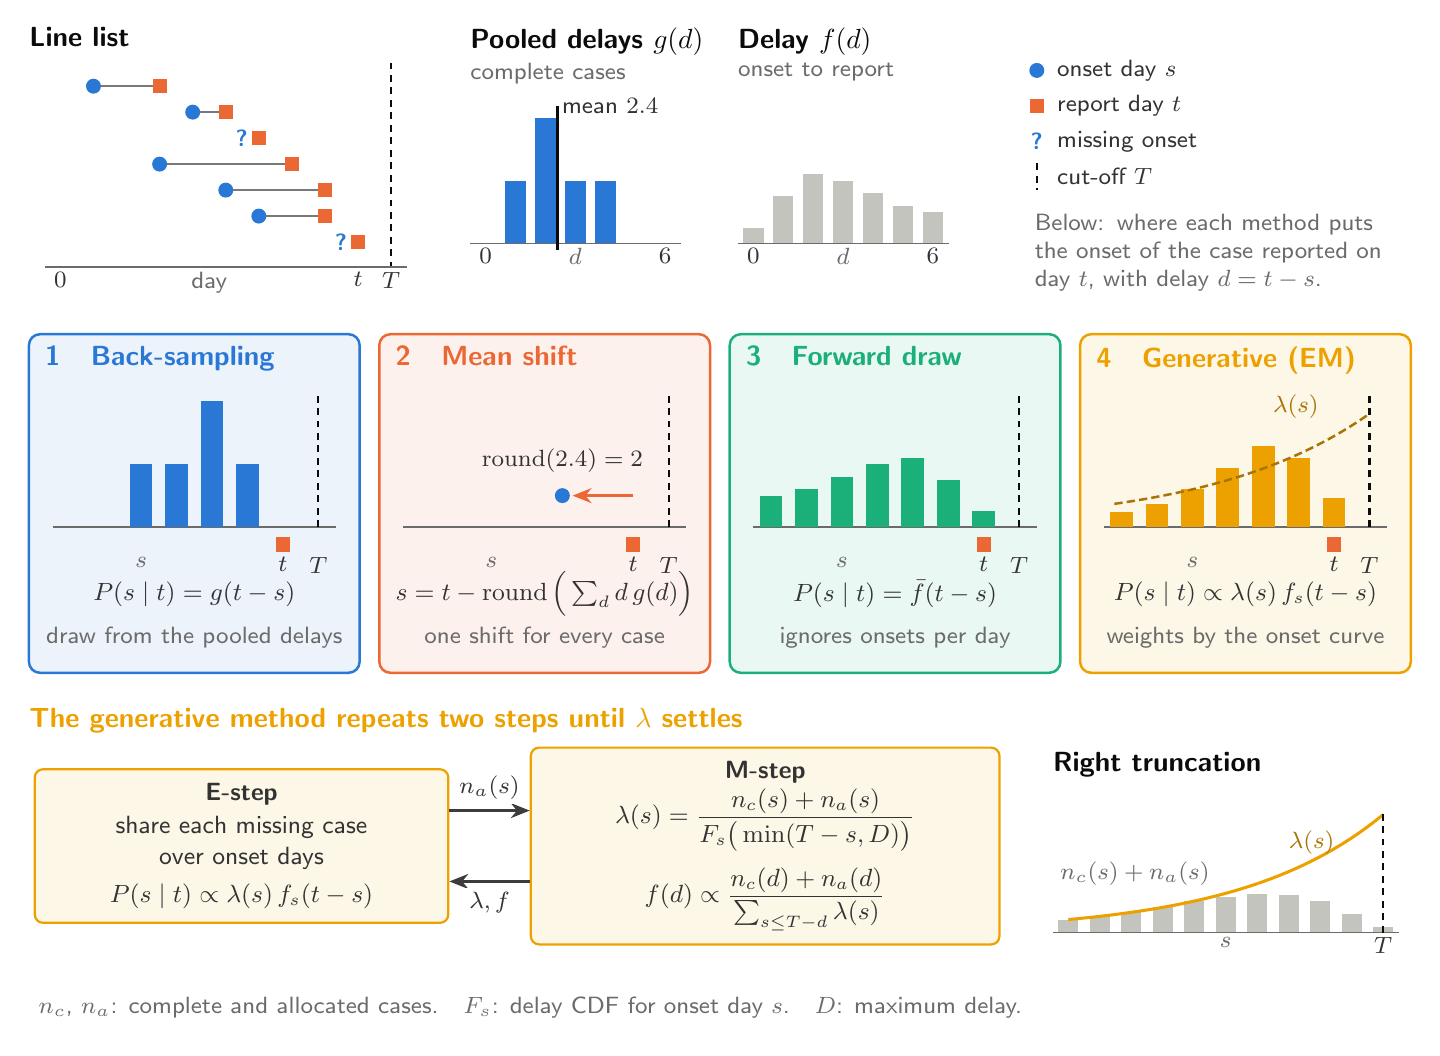
\begin{tikzpicture}[x=1cm,y=1cm]

% ---- Line list -----------------------------------------------------------
% Day d sits at x = 0.4 + 0.42 d; case i on row y = -0.75 - 0.33 i.
\def\dx#1{({0.4+0.42*(#1)})}
\node[paneltitle=ink] at (0,0) {Line list};
\draw[cutoff] ({0.4+0.42*10},-0.45) -- ({0.4+0.42*10},-3.05);
\foreach \i/\s/\t in {0/1/3, 1/4/5, 3/3/7, 4/5/8, 5/6/8} {
  \draw[link] ({0.4+0.42*\s},{-0.75-0.33*\i}) --
    ({0.4+0.42*\t},{-0.75-0.33*\i});
  \node[onset] at ({0.4+0.42*\s},{-0.75-0.33*\i}) {};
  \node[report] at ({0.4+0.42*\t},{-0.75-0.33*\i}) {};
}
\foreach \i/\t in {2/6, 6/9} {
  \node[report] (r\i) at ({0.4+0.42*\t},{-0.75-0.33*\i}) {};
  \node[font=\footnotesize\bfseries, text=onsetcol, left=1pt of r\i,
    inner sep=0pt] {?};
}
\draw[axis] (0.2,-3.05) -- (4.8,-3.05);
\foreach \d/\l in {0/0, 9/t, 10/T}
  \node[label, anchor=north] at ({0.4+0.42*\d},-3.05) {$\l$};
\node[label, text=muted, anchor=north] at ({0.4+0.42*4.5},-3.05) {day};

% ---- Delays --------------------------------------------------------------
% Delay d sits at x = x0 + 0.38 d; probability p has height 4p.
\node[paneltitle=ink] at (5.6,0) {Pooled delays $g(d)$};
\node[note, anchor=north west, inner sep=0pt] at (5.6,-0.45)
  {complete cases};
\begin{scope}[shift={(5.8,-2.75)}]
  \foreach \d/\p in {1/0.2, 2/0.4, 3/0.2, 4/0.2}
    \fill[bar=bscol] ({0.38*\d-0.13},0) rectangle ({0.38*\d+0.13},{4*\p});
  \draw[axis] (-0.2,0) -- ({0.38*6+0.2},0);
  \draw[line width=0.8pt, draw=ink] ({0.38*2.4},-0.08) -- ({0.38*2.4},1.75);
  \node[label, anchor=west] at ({0.38*2.4},1.75) {mean $2.4$};
  \foreach \d in {0,6}
    \node[label, anchor=north] at ({0.38*\d},0) {$\d$};
  \node[label, text=muted, anchor=north] at ({0.38*3},0) {$d$};
\end{scope}

\node[paneltitle=ink] at (9.0,0) {Delay $f(d)$};
\node[note, anchor=north west, inner sep=0pt] at (9.0,-0.45)
  {onset to report};
\begin{scope}[shift={(9.2,-2.75)}]
  \foreach \d/\p in {0/0.05, 1/0.15, 2/0.22, 3/0.20, 4/0.16, 5/0.12, 6/0.10}
    \fill[bar=barcol] ({0.38*\d-0.13},0) rectangle ({0.38*\d+0.13},{4*\p});
  \draw[axis] (-0.2,0) -- ({0.38*6+0.2},0);
  \foreach \d in {0,6}
    \node[label, anchor=north] at ({0.38*\d},0) {$\d$};
  \node[label, text=muted, anchor=north] at ({0.38*3},0) {$d$};
\end{scope}

% ---- Key -----------------------------------------------------------------
\begin{scope}[shift={(12.7,-0.55)}]
  \node[onset] at (0.1,0) {};
  \node[label, anchor=west] at (0.3,0) {onset day $s$};
  \node[report] at (0.1,-0.45) {};
  \node[label, anchor=west] at (0.3,-0.45) {report day $t$};
  \node[font=\footnotesize\bfseries, text=onsetcol] at (0.1,-0.9) {?};
  \node[label, anchor=west] at (0.3,-0.9) {missing onset};
  \draw[cutoff] (0.1,-1.18) -- (0.1,-1.52);
  \node[label, anchor=west] at (0.3,-1.35) {cut-off $T$};
  \node[note, anchor=north west, text width=4.6cm, align=left]
    at (-0.05,-1.7) {Below: where each method puts\\ the onset of the case
    reported on\\ day $t$, with delay $d = t - s$.};
\end{scope}

% ---- Method panels -------------------------------------------------------
% Panel i spans x = 4.45 i to 4.45 i + 4.2. In each plot day s sits at
% u = s - 2.5 with 0.45 cm per day, and probability p has height 4p.
\def\ptop{-3.9}
\def\yb{-6.35}

% #1 index, #2 colour, #3 title.
\newcommand{\methodpanel}[3]{%
  \fill[panel=#2] ({4.45*#1},\ptop) rectangle ({4.45*#1+4.2},{\yb-1.85});
  \node[paneltitle=#2] at ({4.45*#1+0.2},{\ptop-0.15}) {#3};
  \begin{scope}[shift={({4.45*#1+0.3},\yb)}, x=0.45cm, y=4cm]
    \draw[axis] (0,0) -- (8,0);
    \draw[cutoff] (7.5,0) -- (7.5,0.42);
    \node[report] at (6.5,-0.055) {};
    \node[label, anchor=north] at (6.5,-0.08) {$t$};
    \node[label, anchor=north] at (7.5,-0.08) {$T$};
    \node[label, text=muted, anchor=north] at (2.5,-0.08) {$s$};
  \end{scope}}

% #1 index, #2 text.
\newcommand{\panelmaths}[2]{%
  \node[anchor=center] at ({4.45*#1+2.1},{\yb-0.85}) {#2};}
\newcommand{\panelnote}[2]{%
  \node[note, anchor=center] at ({4.45*#1+2.1},{\yb-1.4}) {#2};}

% 1. Back-sampling.
\methodpanel{0}{bscol}{1\quad Back-sampling}
\begin{scope}[shift={(0.3,\yb)}, x=0.45cm, y=4cm]
  \foreach \s/\p in {8/0.2, 7/0.4, 6/0.2, 5/0.2}
    \fill[bar=bscol] ({\s-2.5-0.32},0) rectangle ({\s-2.5+0.32},\p);
\end{scope}
\panelmaths{0}{$P(s \mid t) = g(t - s)$}
\panelnote{0}{draw from the pooled delays}

% 2. Mean shift.
\methodpanel{1}{meancol}{2\quad Mean shift}
\begin{scope}[shift={(4.75,\yb)}, x=0.45cm, y=4cm]
  \draw[flow, draw=meancol, shorten >=1.3mm] (6.5,0.1) -- (4.5,0.1);
  \node[onset] at (4.5,0.1) {};
  \node[label, anchor=south] at (4.5,0.16) {$\operatorname{round}(2.4) = 2$};
\end{scope}
\panelmaths{1}{$s = t - \operatorname{round}\Big(\sum_d d \, g(d)\Big)$}
\panelnote{1}{one shift for every case}

% 3. Forward draw.
\methodpanel{2}{fwdcol}{3\quad Forward draw}
\begin{scope}[shift={(9.2,\yb)}, x=0.45cm, y=4cm]
  \foreach \s/\p in {9/0.05, 8/0.15, 7/0.22, 6/0.20, 5/0.16, 4/0.12, 3/0.10}
    \fill[bar=fwdcol] ({\s-2.5-0.32},0) rectangle ({\s-2.5+0.32},\p);
\end{scope}
\panelmaths{2}{$P(s \mid t) = \bar f(t - s)$}
\panelnote{2}{ignores onsets per day}

% 4. Generative EM.
\methodpanel{3}{gencol}{4\quad Generative (EM)}
\begin{scope}[shift={(13.65,\yb)}, x=0.45cm, y=4cm]
  \foreach \s/\p in {9/0.091, 8/0.219, 7/0.258, 6/0.188, 5/0.121, 4/0.073,
      3/0.049}
    \fill[bar=gencol] ({\s-2.5-0.32},0) rectangle ({\s-2.5+0.32},\p);
  \draw[line width=0.9pt, draw=gencol!70!ink, dash pattern=on 3pt off 1.5pt,
    domain=0.3:7.5, samples=40, smooth]
    plot (\x, {0.36*exp(0.22*(\x-7.5))});
  \node[label, text=gencol!70!ink, anchor=south east] at (6.2,0.33) {$\lambda(s)$};
\end{scope}
\panelmaths{3}{$P(s \mid t) \propto \lambda(s) \, f_s(t - s)$}
\panelnote{3}{weights by the onset curve}

% ---- EM loop -------------------------------------------------------------
\def\ytop{-8.65}
\node[paneltitle=gencol] at (0,\ytop)
  {The generative method repeats two steps until $\lambda$ settles};

\node[box=gencol, text width=4.9cm] (estep) at (2.7,-10.4)
  {\textbf{E-step}\\[1pt] share each missing case\\ over onset days\\[3pt]
   $P(s \mid t) \propto \lambda(s) \, f_s(t - s)$};
\node[box=gencol, text width=5.6cm] (mstep) at (9.35,-10.4)
  {\textbf{M-step}\\[1pt]
   $\lambda(s) = \dfrac{n_c(s) + n_a(s)}{F_s\big(\min(T - s, D)\big)}$\\[5pt]
   $f(d) \propto \dfrac{n_c(d) + n_a(d)}{\sum_{s \le T - d} \lambda(s)}$};
\draw[flow] ([yshift=0.45cm]estep.east) -- ([yshift=0.45cm]mstep.west)
  node[edgelabel, midway, above=2pt] {$n_a(s)$};
\draw[flow] ([yshift=-0.45cm]mstep.west) -- ([yshift=-0.45cm]estep.east)
  node[edgelabel, midway, below=2pt] {$\lambda, f$};

% Right truncation: counts so far fall near T; lambda divides them by F.
% Day s sits at 0.4 s, lambda(s) = exp(0.22 (s - 10)) has height 1.5.
\node[paneltitle=ink] at (13.0,{\ytop-0.55}) {Right truncation};
\begin{scope}[shift={(13.2,-11.5)}, x=0.4cm, y=1.5cm]
  \foreach \s/\n in {0/0.111, 1/0.138, 2/0.172, 3/0.214, 4/0.267, 5/0.300,
      6/0.324, 7/0.321, 8/0.270, 9/0.161, 10/0.050}
    \fill[bar=barcol] ({\s-0.32},0) rectangle ({\s+0.32},\n);
  \draw[line width=1.1pt, draw=gencol, domain=0:10, samples=40, smooth]
    plot (\x, {exp(0.22*(\x-10))});
  \draw[axis] (-0.5,0) -- (10.5,0);
  \draw[cutoff] (10,0) -- (10,1.05);
  \node[label, anchor=north] at (10,0) {$T$};
  \node[label, text=muted, anchor=north] at (5,0) {$s$};
  \node[label, text=gencol!70!ink, anchor=south east] at (8.6,0.62)
    {$\lambda(s)$};
  \node[label, text=muted, anchor=south west] at (-0.4,0.36)
    {$n_c(s) + n_a(s)$};
\end{scope}

\node[note, anchor=north west, align=left] at (0,-12.2)
  {$n_c$, $n_a$: complete and allocated cases.\quad
   $F_s$: delay CDF for onset day $s$.\quad
   $D$: maximum delay.};

\end{tikzpicture}
\end{document}
